% ============================================================
\chapter{Motivations et Vue d'Ensemble}
\label{ch:motivations}
% ============================================================

Imaginez un nuage de points dans un espace de grande dimension. Les
statistiques classiques vous donneront sa moyenne, sa variance, ses
composantes principales. Mais elles ne vous diront pas s'il y a un
\og trou\fg{} au milieu, une boucle, ou deux amas s\'epar\'es par un vide.
Ces caract\'eristiques \emph{topologiques} --- la forme globale des donn\'ees
--- sont pourtant souvent les plus informatives. C'est l'intuition
fondatrice de l'\emph{analyse topologique des donn\'ees} (TDA), un domaine
n\'e au d\'ebut des ann\'ees 2000 des travaux de Gunnar Carlsson, Herbert
Edelsbrunner et d'autres, \`a la fronti\`ere entre la topologie alg\'ebrique,
la g\'eom\'etrie computationnelle et la science des donn\'ees.

\begin{intuition}
Pourquoi avons-nous besoin de la topologie pour analyser des donn\'ees~?
Parce que la \emph{forme} des donn\'ees --- leurs trous, leurs composantes
connexes, leurs cavit\'es --- porte une information que les statistiques
classiques ne capturent pas.
\end{intuition}

% ============================================================
\section{Le probl\`eme fondamental}
% ============================================================

Consid\'erons un nuage de $n$ points $X = \{x_1, \ldots, x_n\} \subset \R^d$.
Ce nuage est souvent un \'echantillon bruit\'e d'un espace topologique
sous-jacent $\mathcal{M}$ (une vari\'et\'e, une courbe, une surface\ldots).
Le probl\`eme central de la TDA est~:

\begin{formules}[title=\textbf{Question fondamentale}]
\emph{Comment r\'ecup\'erer les propri\'et\'es topologiques de $\mathcal{M}$
\`a partir de l'\'echantillon fini $X$~?}
\end{formules}

\begin{exemple}
Soit $\mathcal{M} = S^1$ le cercle unit\'e dans $\R^2$. Un \'echantillon
de $100$ points bruit\'es sur ce cercle forme un anneau. Topologiquement,
$S^1$ poss\`ede une composante connexe ($\beta_0 = 1$) et un trou
($\beta_1 = 1$). La TDA permet de retrouver ces invariants \`a partir
du nuage de points.
\end{exemple}

% ============================================================
\section{Limites des approches classiques}
% ============================================================

Les m\'ethodes statistiques et d'apprentissage classiques pr\'esentent
plusieurs limitations face aux donn\'ees de forme complexe~:

\begin{enumerate}
  \item \textbf{Sensibilit\'e au syst\`eme de coordonn\'ees}~: les
        statistiques descriptives (moyenne, variance) d\'ependent du
        rep\`ere choisi. La topologie est invariante par hom\'eomorphisme.
  \item \textbf{Perte d'information structurelle}~: le clustering
        identifie des composantes connexes mais ignore les trous et
        cavit\'es.
  \item \textbf{Fl\'eau de la dimension}~: en haute dimension, les
        distances euclidiennes deviennent peu informatives, mais les
        invariants topologiques restent significatifs.
  \item \textbf{Absence de multi-\'echelle}~: fixer un seuil de distance
        est arbitraire~; la persistance explore \emph{toutes} les
        \'echelles simultan\'ement.
\end{enumerate}

% ============================================================
\section{La philosophie de la TDA}
% ============================================================

La TDA repose sur trois principes directeurs~:

\begin{definition}[Principes de la TDA]
\begin{enumerate}
  \item \textbf{Invariance par d\'eformation}~: les propri\'et\'es
        topologiques sont pr\'eserv\'ees par d\'eformation continue
        (hom\'eomorphisme, \'equivalence d'homotopie).
  \item \textbf{Approche multi-\'echelle}~: plut\^ot que de fixer un
        param\`etre de r\'esolution, on \'etudie l'\'evolution de la
        topologie sur tout le spectre de r\'esolutions.
  \item \textbf{Stabilit\'e}~: de petites perturbations des donn\'ees
        produisent de petites perturbations des descripteurs topologiques.
\end{enumerate}
\end{definition}

% ============================================================
\section{Illustration visuelle : du nuage au complexe}
% ============================================================

La construction fondamentale de la TDA consiste \`a \'epaissir
progressivement un nuage de points en un objet g\'eom\'etrique dont on
peut calculer la topologie.

\begin{center}
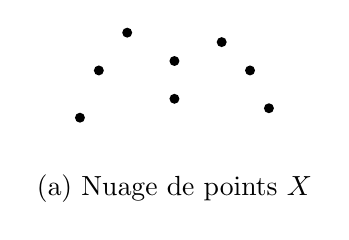
\begin{tikzpicture}[scale=1.2]
  % Points
  \foreach \p in {(0,0),(1,0.2),(0.5,0.9),(1.5,0.8),(2,0.1),
                  (0.2,0.5),(1.8,0.5),(1,0.6)}{
    \fill \p circle (1.5pt);
  }
  \node[below] at (1,-0.5) {(a) Nuage de points $X$};
\end{tikzpicture}
\hspace{1cm}
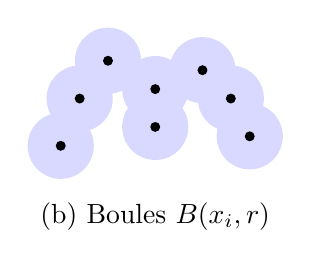
\begin{tikzpicture}[scale=1.2]
  % Points with balls
  \foreach \p in {(0,0),(1,0.2),(0.5,0.9),(1.5,0.8),(2,0.1),
                  (0.2,0.5),(1.8,0.5),(1,0.6)}{
    \fill[blue!15] \p circle (0.35);
    \fill \p circle (1.5pt);
  }
  \node[below] at (1,-0.5) {(b) Boules $B(x_i, r)$};
\end{tikzpicture}
\hspace{1cm}
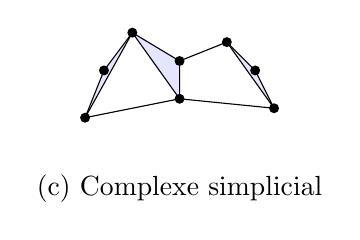
\begin{tikzpicture}[scale=1.2]
  % Simplicial complex
  \fill[blue!10] (0,0) -- (0.2,0.5) -- (0.5,0.9) -- cycle;
  \fill[blue!10] (0.5,0.9) -- (1,0.6) -- (1,0.2) -- cycle;
  \fill[blue!10] (1.5,0.8) -- (1.8,0.5) -- (2,0.1) -- cycle;
  \draw (0,0) -- (1,0.2) -- (0.5,0.9) -- cycle;
  \draw (0,0) -- (0.2,0.5) -- (0.5,0.9);
  \draw (1,0.2) -- (1,0.6) -- (1.5,0.8);
  \draw (1,0.6) -- (0.5,0.9);
  \draw (1.5,0.8) -- (1.8,0.5) -- (2,0.1);
  \draw (1,0.2) -- (2,0.1);
  \draw (1.5,0.8) -- (2,0.1);
  \foreach \p in {(0,0),(1,0.2),(0.5,0.9),(1.5,0.8),(2,0.1),
                  (0.2,0.5),(1.8,0.5),(1,0.6)}{
    \fill \p circle (1.5pt);
  }
  \node[below] at (1,-0.5) {(c) Complexe simplicial};
\end{tikzpicture}
\end{center}

% ============================================================
\section{Nombres de Betti : une premi\`ere intuition}
% ============================================================

Les nombres de Betti sont les invariants topologiques les plus simples.
Intuitivement~:

\begin{formules}[title=\textbf{Nombres de Betti}]
\begin{align}
\beta_0 &= \text{nombre de composantes connexes} \\
\beta_1 &= \text{nombre de trous (boucles)} \\
\beta_2 &= \text{nombre de cavit\'es (vides enclos)} \\
\beta_p &= \text{nombre de ``trous'' de dimension } p
\end{align}
\end{formules}

\begin{exemple}
\begin{itemize}
  \item Un disque plein~: $\beta_0 = 1$, $\beta_1 = 0$.
  \item Un cercle $S^1$~: $\beta_0 = 1$, $\beta_1 = 1$.
  \item Un tore $T^2$~: $\beta_0 = 1$, $\beta_1 = 2$, $\beta_2 = 1$.
  \item Une sph\`ere $S^2$~: $\beta_0 = 1$, $\beta_1 = 0$,
        $\beta_2 = 1$.
\end{itemize}
\end{exemple}

% ============================================================
\section{Pipeline typique de la TDA}
% ============================================================

Le processus g\'en\'eral d'analyse topologique suit les \'etapes~:

\begin{algorithme}[title=\textbf{Pipeline TDA standard}]
\begin{enumerate}
  \item \textbf{Donn\'ees}~: nuage de points $X \subset \R^d$ ou
        matrice de distances.
  \item \textbf{Filtration}~: construire une famille embo\^{\i}t\'ee de
        complexes simpliciaux $K_{r_1} \subseteq K_{r_2} \subseteq \cdots$.
  \item \textbf{Homologie persistante}~: calculer la naissance et la
        mort de chaque caract\'eristique topologique.
  \item \textbf{Repr\'esentation}~: encoder le r\'esultat en diagramme de
        persistance ou code-barres.
  \item \textbf{Vectorisation}~: transformer en vecteur de
        caract\'eristiques pour l'apprentissage.
  \item \textbf{Analyse/Pr\'ediction}~: appliquer des m\'ethodes
        statistiques ou de ML.
\end{enumerate}
\end{algorithme}

\begin{codeblock}[title=\textbf{Premier exemple avec Ripser}]
\begin{minted}{python}
import numpy as np
from ripser import ripser
import matplotlib.pyplot as plt
from persim import plot_diagrams

# Générer un cercle bruité
theta = np.linspace(0, 2*np.pi, 100, endpoint=False)
X = np.column_stack([np.cos(theta), np.sin(theta)])
X += 0.1 * np.random.randn(*X.shape)

# Calculer l'homologie persistante
result = ripser(X, maxdim=1)
diagrams = result['dgms']

# Visualiser
fig, axes = plt.subplots(1, 2, figsize=(12, 5))
axes[0].scatter(X[:, 0], X[:, 1], s=10)
axes[0].set_title("Nuage de points")
axes[0].set_aspect('equal')
plot_diagrams(diagrams, ax=axes[1])
axes[1].set_title("Diagramme de persistance")
plt.tight_layout()
plt.savefig("premier_exemple_tda.pdf")
\end{minted}
\end{codeblock}

% ============================================================
\section{Aper\c{c}u des applications}
% ============================================================

La TDA a d\'emontr\'e son utilit\'e dans de nombreux domaines~:

\subsection{Biologie et m\'edecine}
\begin{itemize}
  \item \textbf{Analyse de la forme des prot\'eines}~: les nombres de
        Betti persistants caract\'erisent les cavit\'es et tunnels des
        structures mol\'eculaires.
  \item \textbf{G\'enomique}~: Mapper r\'ev\`ele des sous-groupes dans
        les donn\'ees d'expression g\'enique du cancer du sein.
  \item \textbf{Imagerie m\'edicale}~: d\'etection de tumeurs via
        l'homologie persistante des images.
\end{itemize}

\subsection{Neurosciences}
\begin{itemize}
  \item \textbf{Connectome c\'er\'ebral}~: analyse topologique des
        r\'eseaux neuronaux.
  \item \textbf{Codes neuronaux}~: l'homologie persistante r\'ev\`ele
        la structure des repr\'esentations spatiales (cellules de lieu).
\end{itemize}

\subsection{Science des mat\'eriaux}
\begin{itemize}
  \item \textbf{Mat\'eriaux amorphes}~: caract\'erisation de la
        structure \`a moyenne port\'ee.
  \item \textbf{Mat\'eriaux poreux}~: quantification de la porosit\'e
        via les nombres de Betti.
\end{itemize}

\subsection{Donn\'ees temporelles et signaux}
\begin{itemize}
  \item \textbf{D\'etection d'anomalies}~: les changements topologiques
        signalent des r\'egimes anormaux.
  \item \textbf{Reconstruction de Takens}~: plongement d'une s\'erie
        temporelle et analyse de la forme r\'esultante.
\end{itemize}

% ============================================================
\section{Formalisme math\'ematique~: un premier aper\c{c}u}
% ============================================================

Nous terminons ce chapitre d'introduction par un aper\c{c}u formel des
objets principaux, qui seront d\'evelopp\'es dans les chapitres suivants.

\begin{definition}[Filtration]
Une \emph{filtration} est une famille de sous-espaces topologiques
(ou de complexes simpliciaux) $\{K_r\}_{r \in \R}$ telle que~:
\[
  r \leq s \implies K_r \subseteq K_s.
\]
\end{definition}

\begin{definition}[Module de persistance]
Un \emph{module de persistance} est un foncteur
$\mathbf{V} : (\R, \leq) \to \mathbf{Vec}_\mathbb{F}$ qui associe \`a
chaque $r \in \R$ un espace vectoriel $V_r$ et \`a chaque paire $r \leq s$
une application lin\'eaire $v_r^s : V_r \to V_s$.
\end{definition}

\begin{theoreme}[D\'ecomposition des modules de persistance]
Tout module de persistance \emph{pointwise finite-dimensional} (p.f.d.)
se d\'ecompose de mani\`ere unique (\`a isomorphisme pr\`es) en somme
directe de modules d'intervalle~:
\[
  \mathbf{V} \cong \bigoplus_{j \in J} \mathbb{I}[b_j, d_j)
\]
o\`u $\mathbb{I}[b,d)$ est le module qui vaut $\mathbb{F}$ sur $[b,d)$
et $0$ ailleurs, avec applications identit\'e sur l'intervalle.
\end{theoreme}

% ============================================================
\section{Pourquoi la topologie et pas seulement la g\'eom\'etrie~?}
% ============================================================

\begin{remarque}
La g\'eom\'etrie \'etudie des propri\'et\'es m\'etriques (distances,
courbures, angles) qui d\'ependent du plongement. La topologie \'etudie
des propri\'et\'es invariantes par d\'eformation continue~: elle est plus
grossi\`ere mais plus robuste. La TDA exploite cette robustesse pour
extraire l'information essentielle.

Par exemple, une tasse et un beignet sont topologiquement identiques
(tous deux ont un trou), bien qu'ils soient g\'eom\'etriquement tr\`es
diff\'erents.
\end{remarque}

% ============================================================
\section{Exercices}
% ============================================================

\begin{exercice}
G\'en\'erer un nuage de $200$ points \'echantillonn\'es uniform\'ement
sur un tore dans $\R^3$ (param\'etrisation standard avec $R=2, r=1$).
Ajouter un bruit gaussien de variance $\sigma^2 = 0.05$. Calculer
l'homologie persistante avec \texttt{ripser} et v\'erifier que l'on
retrouve $\beta_0 = 1$, $\beta_1 = 2$, $\beta_2 = 1$.
\end{exercice}

\begin{exercice}
Expliquer pourquoi les nombres de Betti seuls ne suffisent pas \`a
distinguer tous les espaces topologiques. Donner un exemple de deux
espaces ayant les m\^emes nombres de Betti mais qui ne sont pas
hom\'eomorphes.
\end{exercice}

\begin{exercice}
Impl\'ementer le calcul na\"{\i}f de la matrice de distances deux \`a
deux pour un nuage de $n$ points dans $\R^d$. Quelle est la
complexit\'e~? Comment cette matrice est-elle utilis\'ee dans la
construction d'un complexe de Vietoris--Rips~?
\end{exercice}

\begin{exercice}
Rechercher dans la litt\'erature un article r\'ecent (post-2020)
utilisant la TDA dans un domaine d'application de votre choix.
R\'esumer la m\'ethodologie en une page~: quelles donn\'ees, quel
complexe, quels descripteurs topologiques, quel r\'esultat principal~?
\end{exercice}
